\chapter{Social Networks}

The next day, Rishnak was talking with his ghost friends about his mathematical adventures with Ajur. Seeing Ajur and Jura approach, Rishnak cut short his conversation and joined Ajur and Jura.

Rishnak started the session right away. He said, ``Over the last century, applications of graph theory abound in such fields as engineering, physics, and anywhere there is a need for optimization. More recently, though, with the prolific use of social network applications, including Facebook, Twitter, and LinkedIn, sociologists and psychologists have also found graph theory methods quite useful in their work''

Ajur nodded his head and said, ``Sure, like how we are all so well-connected.  Groups of friends. I remember we talked about cliques awhile ago.''

Rishnak said, ``Exactly. Stanley Milgram, a famous psychologist, wanted to show that people were well-connected. He devised an experiment in which he selected a collection of people living in the Midwestern United States. He asked them to send postcards to a single person~$P$ in Boston. And if they did not know person~$P$ then they could send a postcard to a person that knows someone who knows person~$P$. The result of this experiment showed that most of the letters reached person~$P$ in five or six steps. Does that remind you of a graph theory concept, Ajur?''

Ajur frowned and thought for a few moments. Then it came to him and he said, ``Aha, yes, this experiment shows that the diameter of this network of people is very small, just about five or six, as you said.''

Rishnak said, ``Precisely. The diameter of this social network tells us the longest of all of the shortest distances between any pair of vertices. Social networks have also been used in studying connections within a network of actors and actresses. Actors and actresses form the vertices, and we add edges between vertices if the corresponding actors or actresses have acted in the same film. Have you ever heard of Kevin Bacon?''

Ajur said, ``Kevin who?''

Rishnak rolled his eyes, then said, ``There is an actor by the name of Kevin Bacon who has acted with many other actors and actresses over the years. Many would ask what their Kevin Bacon distance was! It is essentially the length of the path from the person asking the question to Kevin Bacon in the co-actor network. There is even a dedicated website for finding these paths.\footnote{Have a look at \url{http://oracleofbacon.org/movielinks.php}.} And a play about this concept of \textit{six degrees of separation}. Just like Milgram's experiment, this Kevin Bacon network shows that the diameter of the network is very small and there is a Kevin Bacon vertex with a large degree.''

Ajur laughed at this, though was also intrigued by the resulting diameter being very small in comparison to the vast number of vertices in the network or graph.

Rishnak continued, ``Social networks have also been identified in co-author networks for authors of scientific and mathematical publications. Remember Paul Erd\H{o}s? He was a famous twentieth century mathematician and a prolific contributor to the field of graph theory. He wrote so many papers with so many different co-authors that the concept of an Erd\H{o}s distance was defined. Here, authors are vertices and two vertices (or authors) are connected by an edge if they have written a paper together. The American Mathematical Society has a website that calculates this Erd\H{o}s distance to other authors.\footnote{See \url{https://mathscinet.ams.org/mathscinet/collaborationDistance.html}.}''

Ajur said, ``Is the diameter of that graph also very small?''

Rishnak nodded and said, ``Usually the Erd\H{o}s distance to other graph theorists is a very small number because of the collaborative nature of the work and of course an author like Paul Erd\H{o}s wrote such a large number of papers with a large number of co-authors.''

Ajur said, ``So the vertex corresponding to Erd\H{o}s has a very large degree.''

Rishnak smiled and said, ``Exactly.''

Ajur asked, ``What other social networks are there?''

Rishnak frowned and said, ``Well, while social networks have been used to spread real news, they have also been abused to spread rumors and disinformation called fake news. The news---both real and fake---about individuals or political parties can be spread or shared very easily with one's friends and then one's friends of friends until eventually it covers more or all of the social network. Most fake news items are generated by bots, an abbreviated term for a computer program. And advances in image and audio manipulation make it nearly impossible to distinguish between what is real and what is fake.''

Ajur thought about this for a few seconds, an uneasy feeling coming over him.

Rishnak sighed and said, ``Here's something a bit more positive and rather interesting. The degree distribution of social networks tend to follow what is called a \textit{power law}. In this chart''---Rishnak waved his hands and a chart appeared [Figure~\ref{21p1}]---``we count the degrees of each vertex in a social network. There are a few vertices with large degrees (on the left) and a very large number of vertices with small degrees that form a long tail on the right.''

Ajur thought further about this and said, ``And the vertices with large degrees have many adjacent vertices, so they're like the popular students in school with many friends.''

\begin{figure}
\begin{center}
\includegraphics[width=0.9\textwidth]{degreepowerlawdist.jpg}
\caption{Sample degree distribution of a social network}\label{21p1}
\end{center}

\end{figure}
\begin{newpage}
\end{newpage}
 
Rishnak nodded and said, ``Yes, these individuals are sometimes referred to as hubs.''
 
Thinking about Erd\H{o}s again, Ajur remembered the Erd\H{o}s--R\'enyi model for generating random graphs. He asked, ``Do the Erd\H{o}s--R\'enyi graphs have a uniform degree distribution---I mean all of the vertices have roughly the same degrees?''

Rishnak smiled and said, ``Let me try to explore that further with an example using Facebook. A Facebook graph consists of users as vertices and edges between two users if they are friends of one another---and remember, in Facebook, friendship is a symmetric relationship. It has been found that the average number of Facebook friends per user, which is therefore the average degree of a vertex, is~300 and the median degree is~200.''

Ajur asked, ``How big is the Facebook graph? It must be humongous.''

Rishnak said, ``The Facebook graph has approximately two billion vertices---many of these vertices could be fake users or groups. With a median degree of~200, that means that one billion users have less than~200 friends.''

Ajur raised his eyebrows. He said, ``Wow, that's quite a long tail.''

Rishnak smiled, happy to see Ajur put the various pieces of the puzzle together. He continued, ``And Facebook restricts the maximum number of friends one can have to~5000. According to sociologists, a person can actually be close to at most~150 friends, which tells you something about how close friendships are in Facebook.''

Ajur laughed.

Rishnak continued, ``Also, the Facebook graph has an average separation or diameter of only~3.74.\footnote{\url{https://research.fb.com/blog/2016/02/three-and-a-half-degrees-of-separation/}} There is a well-known Facebook paradox that states that, on average, most people have fewer friends than their friends have. We can see this by studying this graph.'' Rishnak flashed his hands and a graph appeared [Figure~\ref{21g1}].

\begin{figure}
\begin{center}
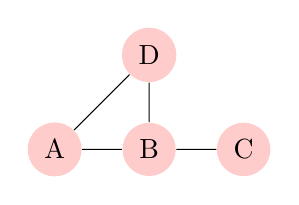
\begin{tikzpicture}
  [scale=.6,auto=left,every node/.style={circle,fill=red!20}]
  \node (n1) at (1,7) {A};
  \node (n2) at (3,7)  {B};
  \node (n3) at (5,7)  {C};
  \node (n4) at (3,9)  {D};

  \foreach \from/\to in {n1/n2,n2/n3,n2/n4,n1/n4}
    \draw (\from) -- (\to);

\end{tikzpicture}
\caption{A graph that explains the Facebook friends paradox}\label{21g1}
\end{center}
\end{figure}

Rishnak said, ``In this graph, the average number of friends---in other words, the average degree---is~$\frac{2+2+3+1}{4}=2$.  Person~$A$ sees that~$D$ has two friends and~$B$ has three friends. Person~$B$ sees that~$A$ and~$D$ both have two friends and~$C$ has only one friend. Person~$C$ sees that~$B$ has three friends. And person~$D$ sees that~$A$ has two friends and~$B$ has three friends. Therefore, the average number of friends one sees is~$\frac{2+3+2+2+1+3+2+3}{8}=2.25$.''

Ajur frowned at this result.

Rishnak continued, ``This is in contradiction to the common belief that one has more friends than their friends have!''

Ajur protested, saying, ``That doesn't make any sense.''

Rishnak laughed and mentioned that there was a nice mathematical explanation for this phenomenon---and that Ajur should discover it on his own.

Kinaja, a glowing white ghost, suddenly appeared. She had been listening to Rishnak go on and on about social networks. She glided in to join them and said, ``I think that virtual social networks, being unregulated, cause a lot of harm---and here are three reasons why:
\begin{enumerate}
    \item Users can too easily be bullied.
    \item Bots and trolls pretend to be genuine users, but they propagate misinformation.
    \item One's private information too easily gets stolen or sold to advertisers.''
\end{enumerate}

Rishnak and Ajur both nodded in agreement.

\subsection*{Question for the nineteenth day}
Rishnak said, ``Ajur, we have come to the nineteenth day. Here is your question. Does the Facebook paradox still hold for a regular graph of degree~3 with 10 vertices?''

\textit{Before you turn the page, try to come up with an answer of your own!}

\newpage
\subsection*{Answer for the nineteenth day}
Ajur worked this problem out by thinking aloud. He said, ``If the degree is~3, then each person will have three friends, but the average number of friends one sees is~$\frac{(3+3+3)*10}{30}=3$. Therefore, for this graph, there will be no paradox.''

Rishnak said, ``Good, Ajur. And note that most real social networks are not regular, so most social networks do see this paradox.''

That was a good place to stop the discussion for the night.
